\documentclass[14pt]{beamer}
\usepackage{beamerthemesplit}
\usetheme{Madrid}
\usefonttheme{serif}
\usepackage{bookman}


\title[SPIN]{Student Performance Information Network}
\author[Damini Charvitha Lendi ]{K. Damini Satya \\K. Sri Charvitha\\M. Lendi Vihari}
\institute[BVRITH]{Department of Information Technology and Computer Science\\II Year\\BVRIT Hyderabad}
\begin{document}

\maketitle

\begin{frame}
\frametitle{Information Overload}
	\begin{columns}[T]
		\begin{column}{.55\textwidth}
		\vspace{8mm}
			Nearly 500 students \\4 branches\\3 programs
				\begin{itemize}
					\item  \pause What is happening? 
					\item How are we doing?
				\end{itemize}
		\end{column}
		\begin{column}{.45\textwidth}
			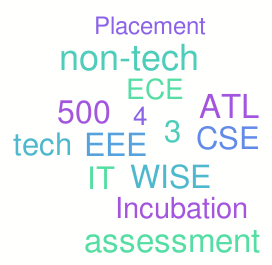
\includegraphics[scale = 0.5]{tag1.png}
		\end{column}
	\end{columns} 
\end{frame}

\begin{frame}
\frametitle{Silver Bullet}
SPIN - A common platform for students and management .
	\begin{center}
		
\includegraphics[scale = 0.4]{interact.jpeg}
	\end{center}
\end{frame}

\begin{frame}
\frametitle{Purpose}
\begin{block}{Student View}
	Get notified with technical and non-technical information.
\end{block}
\begin{block}{Management Perspective}
	\begin{itemize}
		\item Analyse overall performance of students.
		\item Know details of the programs. 
		\item Know the effectiveness of the programs being conducted.
	\end{itemize}
\end{block}
\end{frame}

\begin{frame}{Application Taxonomy}
	\begin{center}
	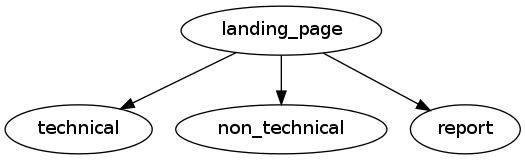
\includegraphics[scale = 0.45]{spin.png}
	\end{center}
\end{frame}

\begin{frame}{Application Taxonomy}
	\begin{center}
	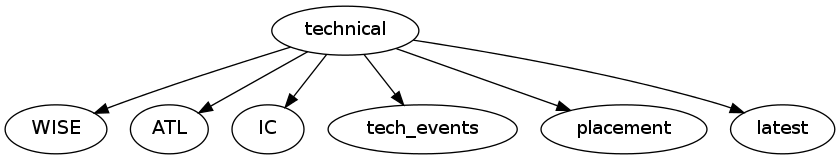
\includegraphics[scale = 0.38]{tech.png}
	\end{center}
\end{frame}

\begin{frame}{Application Taxonomy}
	\begin{center}
	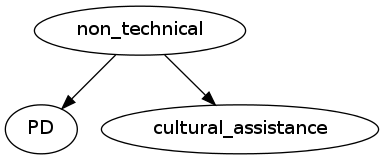
\includegraphics[scale = 0.5]{nontech.png}
	\end{center}
\end{frame}

\begin{frame}{Application Taxonomy}
	\begin{center}
	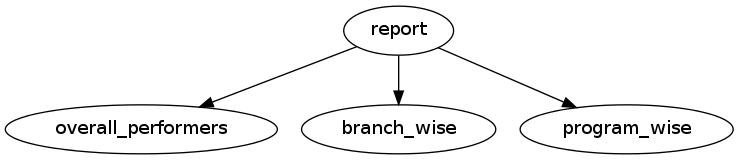
\includegraphics[scale = 0.4]{report.png}
	\end{center}
\end{frame}

\begin{frame}{Modules}
	\begin{block}{Notification Module}
		Notifications Delivered.
	\end{block}
	\begin{block}{Assessment Module}
		Student Achievements showcased.
	\end{block}
	\begin{block}{Admin Module}
		\begin{itemize}
		\item Publish the content to be notified.
		\item Maintain database.
		\end{itemize}
	\end{block}
\end{frame}

\begin{frame}{Flow}
\begin{columns}[T]
		\begin{column}{.5\textwidth}
		\begin{center}
			WISE Notifications
			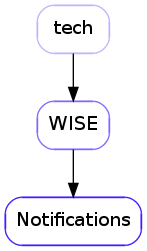
\includegraphics[scale = 0.5]{flow.png}
			\end{center}
		\end{column}
		\begin{column}{.5\textwidth}
		\begin{center}
			CSE Students Info
			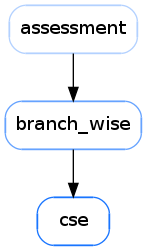
\includegraphics[scale = 0.5]{flow2.png}
			\end{center}
		\end{column}
	\end{columns} 
\end{frame}

\begin{frame}{Learnt}
	\begin{itemize}
		\item Project Development Cycle
		\item Design Database
		\item Servlets
		\item Inotify
		\item Graphviz
		\item Text Processing and Code Generation
	\end{itemize}
	\begin{center}
		\includegraphics[scale=0.35]{insert.png}
	\end{center}
\end{frame}


\begin{frame}{Tools}
	\begin{itemize}
		\item HTML,CSS,JQuery
		\item Servlets
		\item MySQL
		\item File Alteration Monitor
	\end{itemize}
\end{frame}


\begin{frame}{A quick look at the database}
	\begin{center}
		\includegraphics[scale=0.6]{db.png}
	\end{center}
\end{frame}

\begin{frame}{Coming Up}
	\begin{itemize}
		\item Disscussion Fourm
		\item User Posting
	\end{itemize}
\end{frame}

\begin{frame}
	\begin{center}
		
\includegraphics[scale=0.3]{ty.jpg}
	\end{center}
\end{frame}

\end{document}
